\section{First Sketch}

\begin{figure}
%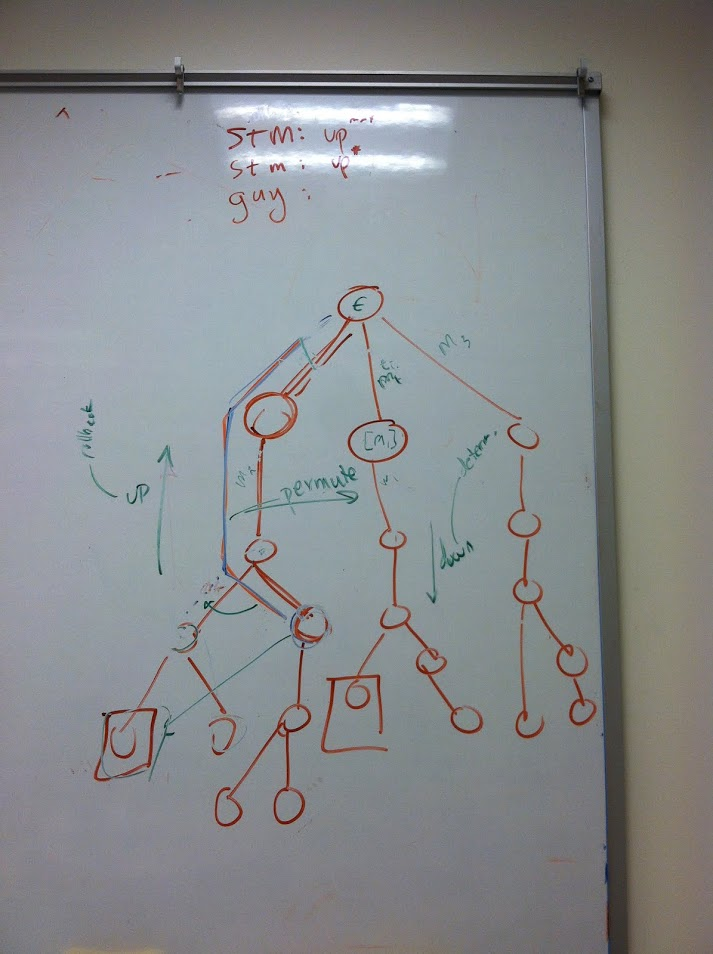
\includegraphics[width=\columnwidth]{tree.jpg}
tree.jpg
\caption{An example}
\label{fig:example}
\end{figure}

We start with a description of all possible interleaved executions of some bounded number of threads, as shown in Figure \ref{fig:example}. Some of the leaf nodes denote admissible final states for the interleaved execution. The rest are inadmissible final states.

A generic concurrent system may produce both admissible and inadmissible executions. Two main approaches have been adopted to produce only admissible executions:
\begin{itemize}
\item apply synchronization to restrict the available parallelism and drive the system only into the admissible executions, and
\item rollback the execution when the system falls into an inadmissible executions, and re-execute the program (sometimes driving the system to avoid to fall back to the inadmissible case already explored).
\end{itemize}

We would like to optimize two properties:
\begin{itemize}
\item Utilization of available parallelism, which is counted as the number of admissible paths that synchronization permits
\item Overhead, which is counted as the number of operation/state reversals that synchronization may force to (re)direct execution toward an admissible final state
\end{itemize}

\todo{for now i guess we just let an operation have unit cost. can
  worry about cost models later}



Our idea is to create a calculus founded on three operations:
\begin{itemize}
\item[Execute] forward execution step
\item[Rollback] local rollback
\item[Permute] a jump to another branch that reflects the same history of operations (but differs in terms of the order of execution of the operations)
\end{itemize}

Once we recognized we fall into an inadmissible execution, our goal is to perform some operations in order to fall into an admissible execution preserving the observable behaviors.
This leads us to two main concepts:
\begin{itemize}
\item What executions are admissible? (in the rest of the paper, we will adopt the classical idea of Software Transaction Memory)
\item What behaviors of an execution are observable? (in the rest of the paper, we will consider final states as the observable behaviors of an execution)
\end{itemize}

We can plug in our approach different definitions of admissible executions, and observable behaviors.

In addition, we want to formalize Permute reaching a node in the tree that is at the same level of the current one. In this way, we do not rollback the execution, but indeed we advance it by one step as we would do if we were in an admissible execution. Intuitively, this means that our permute can be simulated by $n$ rollbacks followed by $m$ execution steps, with $m==n$\footnote{We discussed also the case in which $m>n$, but we are not yet sure if this case will be never interesting}.

\begin{figure}
\begin{lstlisting}
T1:
	put(k,v)
	get(k)

T2:
	remove(k)
\end{lstlisting}
\caption{The running example}
\label{lst:runningexample}
\end{figure}

\begin{figure}[ht]
%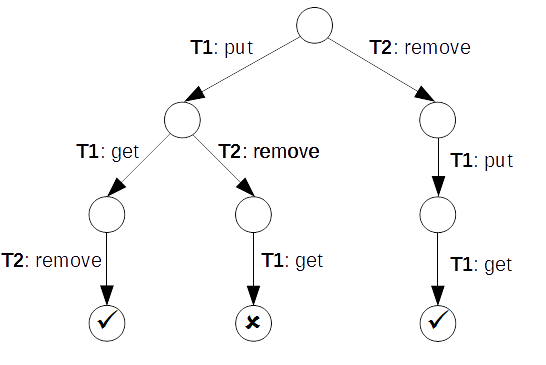
\includegraphics[width=\columnwidth]{treerunningexample.png}
treerunningexample.png
\caption{The tree of executions of the running example}
\label{fig:treerunningexample}
\end{figure}

Consider for instance the running example in Figure \ref{lst:runningexample}.
Figure \ref{fig:treerunningexample} depicts the tree of all possible executions of the running example. We consider the first and last execution as admissible, while the second one is not. This is a quite standard assumption for our running example: The two instructions of T1 conflict with the instruction of T2 (they all work on the same collection and on the same key). Therefore, the system should not allow T2 to execute its instruction if T1 has execute the first instruction but not the second one yet. This is usually achieved in two ways:
\begin{itemize}
\item by synchronization mechanisms (e.g., locks) providing mutual exclusion between T1 and T2, or
\item by rolling back the execution if the system falls into the second path and when executing remove.
\end{itemize}

Instead, we propose a novel approach.
Consider the second path, and the situation in which we have already exposed history \statement{[T1: put, T2: remove]}.
If we refrain from executing remove (that is, we replace it with a skip statement), we would apply a Permute step, that would yield us to the history	\statement{[T2: remove, T1: put]}

In this way, the entire execution becomes \statement{[T2: remove, T1: put, T1: get]} that is an admissible execution.

Note that in contrast with Rollback and Execute, Permute requires an algebraic specification that permits efficient (bounded) editing of the state reflected by \statement{[T1: put, T2: remove]} to arrive at \statement{[T2: remove, T1: put]}.




\section{Permuting the execution -- previous}
The goal of our work is to try to \emph{redirect} a bad execution into a good one by simulating the good trace up to that point. At a given point of an execution, we suppose that we can observe only two things:
\begin{enumerate}
\item where the execution of each transaction is. This can be formalized as $\getTransactionPoints{\tau} = [\statement{t} \mapsto \max(\indexes{\statement{t}}{\tau}) : \statement{t} \in \cset{T}]$
where $\cset{T}$ contains all the identifiers of the transactions in the execution $\tau$, and $\indexes{\statement{t}}{\tau}=\{\cel{i} : \exists \cel{\sigma}_j \to_{(\statement{t}, \cel{i})} \cel{\sigma}_{j+1} \in \tau\}$
\item what we can observe on the last state of the trace. The observational portion of the state is given by a function $\observe{\sigma}$.
\end{enumerate}

Given a bad trace $\sigma_0 \to \cdots \to \sigma_i$ we want to find a good trace $\sigma'_0 \to \cdots \to \sigma'_j$ such that
\begin{enumerate}
\item $\getTransactionPoints{\sigma_0 \to \cdots \to \sigma_i} = \getTransactionPoints{\sigma'_0 \to \cdots \to \sigma'_j}$
\item $\observe{\sigma_0}=\observe{\sigma'_0}$
\item $\observe{\sigma'_j} = \observe{f(\sigma_i)}$ where $f$ is a function that \emph{adjusts} the state of the bad execution to fall into the good execution.
\end{enumerate} 

The two parameters of our framework are $f$ (and a key component is how to compute it) and $\observe{\sigma}$. We suppose that $\observe{\sigma}$ returns the portion of the state that influences what is observable "through" the semantics. This means that if we take two states equivalent modulo observability and we perform the semantics of a statement, we obtain two states that are equivalent modulo observability. Formally,
\[
\begin{array}{c}
\forall \sigma, \sigma' \in \cstates : \observe{\sigma}=\observe{\sigma'} , \forall \statement{s} \in \statements : \langle \statement{s}, \sigma \rangle \to \sigma_1, \langle \statement{s}, \sigma' \rangle \to \sigma'_1\\
\Downarrow\\
\observe{\sigma_1}=\observe{\sigma'_1}\\
\end{array}
\]

Based on the permutation function $f$ we define the semantics $\csemantics{S_{P}}{\statement{p}, \sigma_0}$ that, if the execution falls into a bad trace, redirects the execution into a good trace by applying $f$.\todo{Formalize it, not clear when exactly we apply the permutation}

We can now prove the soundness of our permutation. Intuitively, we prove that if one can observe only the observable part of the entry and the exit state (and not the intermediate state and the interleaving of transactions) it cannot notice the permutation we operate.

\begin{theorem}[Soundness of the permutation]
\[
\forall \sigma_0 \to \cdots \to \sigma_i \in \csemantics{S_{P}}{\statement{p}, \sigma_0}, \exists \sigma_0 \to \cdots \to \sigma'_j \in \csemantics{S}{\statement{p}, \sigma_0} : \observe{\sigma_i} = \observe{\sigma_j}
\]
\todo{Should we relax on the entry state using observe?}
\end{theorem}






\section{New ideas of the meeting on May, 2nd}

\subsection{Observational Equivalence}
Instead of using the idea of an $\mathit{observe}$ function and ask that the states are equal, we can rely on the observational equivalence relation between states. Another approach could be to adopt the POPL 02 Cousot and Cousot framework to define program transformations. First Pietro's intuition: "They deal with online and offline program transformation, and they define observational equivalence as an equivalence among abstractions of concrete executions. Indeed, what we are doing is slightly different: we perform a static analysis offline, and we change the semantics of the program (that - maybe - can be interpreted as a program transformation) online if we fall into a bad execution. On the other hand, I think that we could plug our work into their framework, and the main advantage would be to define the observational equivalence as an abstraction, and in particular as the abstraction we are performing in TVLA. In this way, we won't need to develop an ad-hoc definition of the correspondence between the observational equivalence and what we track with our static analysis."

\subsection{Product of CFGs}
We came up to the idea that in order to represent the interleaving of various threads. If we have two threads T1 and T2, we build up the product of all the nodes, and we add the edges that performs a step in the execution of one of the two threads. In this way we have some spurious paths (e.g., if we are inside a thread performing a loop and we perform one step in the other thread, also this step will be inside the loop), that we should refine through the abstract domain (e.g., adding program pointers of the various threads in the abstract state). In addition, we may have that a bad and a good trace are later joined. In order to distinguish between good and bad traces we will need to partition these two cases in the abstract domain (e.g., through a Bad abstraction predicate in TVLA).

Another idea from Eric was to use his PLDI 09 work (where they perform a sort of loop unrolling by expanding the CFG) but we didn't discuss it in the details.


\section{Cartesian product of transactions}
Given a tuple of $n$ transactions $\cset{T} \in \cfg^n$, we build up the Cartesian product of the cfg of these transactions. Formally, we define the cfg of $\cset{T}$ by $\cel{cfg}_{\cset{T}} = \square_{(\cel{L}_i, \cel{E}_{i}) \in \cset{T}} (\cel{L}_i, \cel{E}_{i})$ where $\square$ denotes the Cartesian product of graphs\todo{Cite something?}. Formally,
\[
\begin{array}{l}
\square_{(\cel{L}_i, \cel{E}_{i}) \in \cset{T}} (\cel{L}_i, \cel{E}_{i}) = (\cel{V}, \cel{E}) :\\
\hspace{20pt} \cel{V}=\Pi_{(\cel{L}_i, \cel{E}_{i}) \in \cset{T}} \cel{L}_i\\
\hspace{20pt} \cel{E}=
\left\{
\begin{array}{l}
(\cel{L}, \cel{L}', \statement{st}) : \cel{L}, \cel{L}' \in \cel{V} \land\\
\hspace{40pt} \exists j \in [1..n] : \forall i \in [1..n] \setminus \{j\}  : \cel{L}_i=\cel{L}'_i \land\\
\hspace{40pt} \exists (\cel{L}_j, \cel{L}'_j, \statement{st}) \in \cel{E}_j\\
\end{array}
\right\}
\end{array}
\]

The intuition behind the Cartesian product of cfgs is that (i) each node represents where the execution of each transaction is arrived, and (ii) each edge represents that one transaction performs the execution of an atomic step, while the others do not progress. In this way, we can rely on the Cartesian product of cfgs to compute the interleaving semantics.

\textbf{Put the running example here}

\subsection{Semantics}
On the Cartesian product of transactions we define the concrete semantics as follows:

\[
\begin{array}{l}
\csemantics{S_{CFG}}{\statement{cfg}_\statement{p}, \sigma_0} = \textit{lfp}_{(\cel{L}_0, \cel{\sigma}_0)}^{\subseteq} \lambda \cset{T} . \cset{T} \cup\\
\hspace{10pt} \left\{
\begin{array}{l}
\hspace{10pt} (\cel{L}_0, \cel{\sigma}_0) \to \cdots \to (\cel{L}_{i-1}, \cel{\sigma}_{i-1}) \to (\cel{L}_i, \cel{\sigma}_i) :\\
\hspace{10pt} (\cel{L}_0, \cel{\sigma}_0) \to \cdots \to (\cel{L}_{i-1}, \cel{\sigma}_{i-1})  \in \cset{T} \land\\
\hspace{10pt} \exists (\cel{L}_{i-1}, \cel{L}_i, \statement{st}) \in \pi_2(\statement{cfg}_\statement{p}) \land (\cel{\sigma}_{i-1}, \statement{st}) \to \cel{\sigma}_i\\
\end{array}
\right\}\\
\end{array}
\]



\begin{lemma}[Soundness of the concrete semantics on the Cartesian product of CFGs]
	$\csemantics{S}{\cel{cfg}_{\cset{T}}, \sigma_0} \subseteq \csemantics{S_{CFG}}{\cel{cfg}_{\cset{T}}, \sigma_0}$
\end{lemma}

\todo{In theory, they are equal and we can prove it, but maybe this is not interesting, maybe yes - it depends if we need an underapproximation for the good traces}

\subsection{Bad flows}
Then we statically detect on the CFG of a set of transactions $\cel{cfg}_{\cset{T}}$ the flows that \emph{may} lead to bad executions. Therefore, we build up a data flow analysis that tracks what actions may reach each label in $\cel{cfg}_{\cset{T}}$.

In particular, we are only interested in triples made by these elements since the properties we want to check are on the last three actions \todo{We should enumerate the 4 cases and cite the work introducing them}. Therefore the abstract domain of our data-flow analysis is $(\labels \cup \{\epsilon\})^3$, where $\epsilon$ represents situation in which we have less than three elements. Our data flow analysis is forward and possible. Therefore, our analysis is defined by the following equations:

$$
\begin{array}{l}
\cfunction{In}(\cel{l}) = \bigcup_{(\cel{l'}, \cel{l}) \in \cel{e}} \cfunction{Out}(\cel{l'})\\
\cfunction{Out}(\cel{l}) = \cfunction{Gen}(\cel{l}) \setminus \cfunction{Kill}(\cel{l}) \\
\cfunction{Kill}(\cel{l}) = \{(\cel{a}_1, \cel{a}_2, \cel{a}_3) : (\cel{a}_1, \cel{a}_2, \cel{a}_3) \in \labels^3\}\\
\cfunction{Gen}(\cel{l}) = \{(\cel{a}_1, \cel{a}_2, \cel{a}_3) : \exists \cel{a}_4 \in \actions \cup \{\epsilon\}: (\cel{a}_2, \cel{a}_3, \cel{a}_4) \in \cfunction{In}(\cel{l}) \land\\
\hspace{125pt} \cel{a}_1 \in \getaction{\cfunction{getWeigth}(\cel{I})} \}
\end{array}
$$

where $\cel{e}$ represents the edges of the cfg, and $\getaction{\statement{st}}{TODO}$ returns the set of actions ($r$ and/or $w$) the given statement may perform.\todo{Since we have the statements of the edges and not in the nodes, the getLabel function is somewhat broken. I should add the out label and the transaction that performs the statement}

Finally, we tag the edges that could expose bad behaviors. For each edge 


In particular, for each edge in $\cel{cfg}_{\cset{T}}$ we consider all the triples of actions generated by this edge. If at least one of these triples represents a conflict, we tag the edge as bad.\todo{Note: we should have one triple per key, but since we are assuming to have only one key statically known we consider this case. This sounds weak}
Bad edges are aimed at over-approximating bad executions.

\begin{theorem}
	$\forall \tau \in \badtraces \cap \csemantics{S}{\statement{p}, \sigma_0} : \tau \in \csemantics{S_C}{\cel{cfg}_{\cset{T}}, \sigma_0} \cap \badtraces$
\end{theorem}

\todo{We should define exactly the semantics over the cartesian product of cfgs and show how the trace is built from there}

